\documentclass[11pt,twocolumn]{article}
\usepackage{enumerate}
\usepackage{hyperref}
\usepackage{amsmath, amssymb, textcomp}
\usepackage{graphicx}
\usepackage[section]{placeins}
\usepackage{cite}

\begin{document}

\title{The Ising model\\ Computational Physics}
\author{Tobias de Jong\\ s0881260}
\date{\today} % Voeg automatisch de datum in

\maketitle
\newcommand{\Part}[3][ ]{\ensuremath{\frac{\partial^{#1} #2}{{\partial #3}^{#1}}}}
\newcommand{\Dif}[3][ ]{\ensuremath{\frac{d^{#1} #2}{{d #3}^{#1}}}}
\renewcommand{\O}[1]{\ensuremath{\mathcal{O}\left(#1\right)}}
\renewcommand{\vec}{\bold}
\section{Introduction}
In this paper we will investigate the different properties of the Ising model in 2D and 3D using Monte Carlo simulation methods. The canonical Metropolis single spin flip method as well as the Wolff cluster flip algorithm are used to obtain values for the critical exponents $\chi$, $\gamma$ and $\nu$ in both 2D and 3D. %for different lattices
\section{Theory}
\subsection{Ising model}
\subsection{Monte Carlo approximation}
\section{Algorithms}
\subsection{Metropolis}
The Metropolis algorithm~\cite{Metropolis} utilizes single spin flips to transition between states. By selecting a random spin at each step we make sure that the transition chance  between any two neighbouring states $\mu$, $\nu$ is equal:
\[g(\mu,\nu) = g(\mu,\nu) = \frac1N\]
\subsection{Wolff}
\section{Implementation}
Both the Metropolis and the Wolff algorithm were implemented using Python and NumPy. While this choice of language will not rersult in the fastest implementation it yields easily readable and adaptable code. Moreover, simple libraries exist to parallelise the different runs to keep the total wall clock computation time reasonable.
\section{Results}
\subsection{Thermalization}
To visualize the thermalisation we do several runs for each value of $\beta$, calculate the magnetisation for each and take the mean across different runs. This way, the plot will be a flat line when thermalized. Results for a $40\times40$ grid and 100 runs per value of beta is given in figure \ref{therm}
\begin{figure}[!ht]
\centering 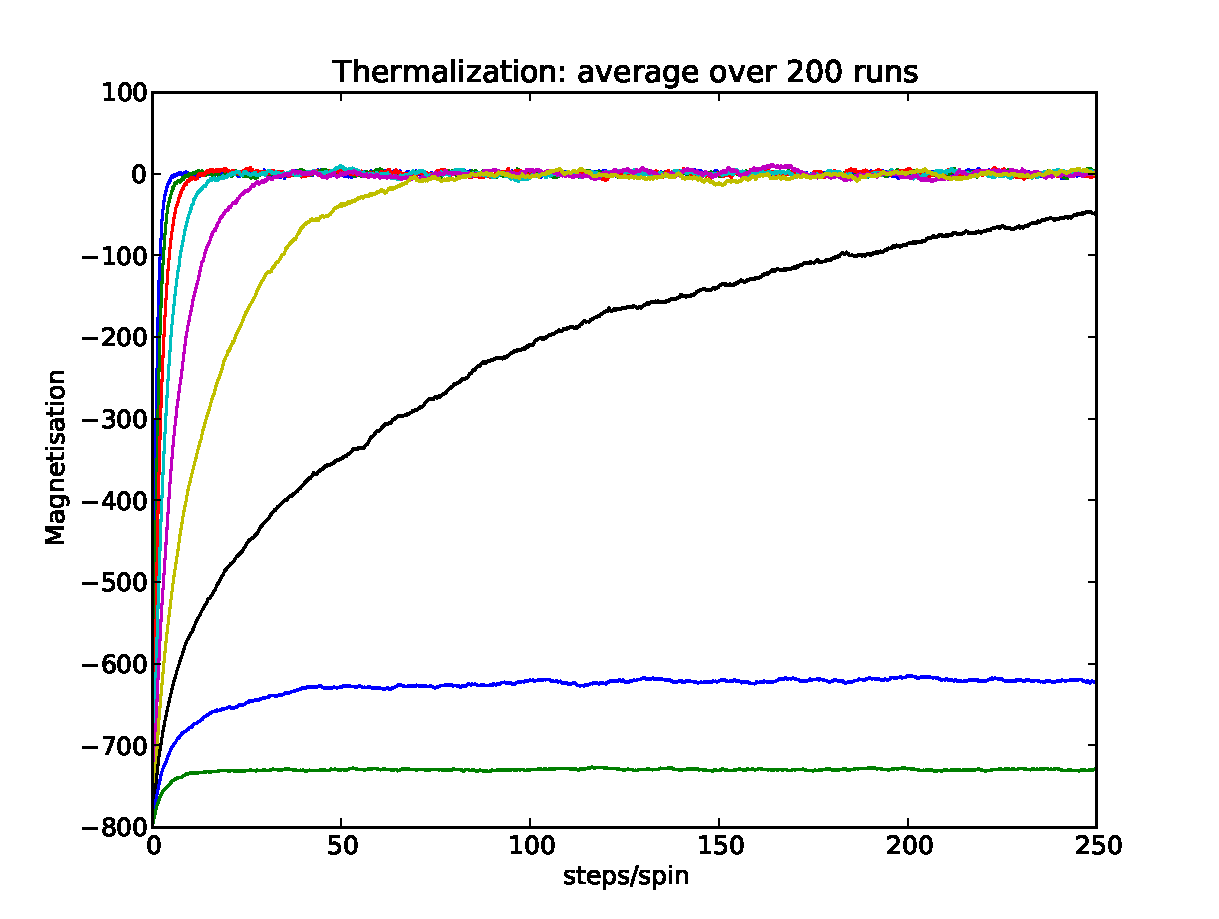
\includegraphics[width=\columnwidth]{figs/therm.pdf}
\caption{Thermalization}
\label{therm}
\end{figure}
\subsection{Auto-correlation}
\subsection{Finite size scaling}
\section{Data collapse}
\bibliography{verslag}{}
\bibliographystyle{plain}


\end{document}
